\begin{figure}[htbp]
	\centering
	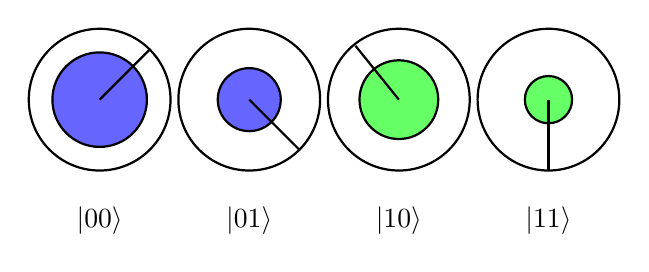
\begin{tikzpicture}[scale=0.95]
		\begin{scope}
			\foreach \x/\label in {0/00, 2/01, 4/10, 6/11} {
				\node[draw, circle, minimum size=1.8cm, thick] (c\x) at (\x,0) {};
			}
			\foreach \x/\fill/\r in {0/blue!60/1.2, 2/blue!60/0.8, 4/green!60/1.0, 6/green!60/0.6} {
				\node[draw, circle, fill=\fill, minimum size=\r cm, thick] at (\x,0) {};
			}
			\draw[thick, black] (0,0) -- (0.68,0.68);
			\draw[thick, black] (2,0) -- (2.68,-0.68);
			\draw[thick, black] (4,0) -- (3.42,0.72);
			\draw[thick, black] (6,0) -- (6.00,-0.96);
			\node[below=0.1cm] at (0,-1.2) {$|00\rangle$};
			\node[below=0.1cm] at (2,-1.2) {$|01\rangle$};
			\node[below=0.1cm] at (4,-1.2) {$|10\rangle$};
			\node[below=0.1cm] at (6,-1.2) {$|11\rangle$};
		\end{scope}
		
	\end{tikzpicture}
	\caption{Two-qubit state in Circle Representation. Circles are arranged in a $2 \times 2$ grid with basis state labels, showing relative amplitudes and phases for each $|ij\rangle$ state. Two-qubit state: Four circles in a $2 \times 2$ grid representing computational basis states $|ij\rangle$.}
	\label{fig:circle-two-qubit}
\end{figure}
